\documentclass[10pt,letterpaper]{article}
\usepackage[utf8]{inputenc}
\usepackage{amsmath}
\usepackage{amsfonts}
\usepackage{amssymb}
\usepackage{graphicx}
\usepackage{etoolbox}
\usepackage{xcolor}
\usepackage{listings}
\usepackage{color}

\title{RBE 595 Motion Planning \\ \large Homework 1}
\author{Daniel Miller}

\definecolor{dkgreen}{rgb}{0,0.6,0}
\definecolor{gray}{rgb}{0.5,0.5,0.5}
\definecolor{mauve}{rgb}{0.58,0,0.82}

\renewcommand{\thesection}{}
\renewcommand{\thesubsection}{}

\setlength{\parskip}{\baselineskip}%
\setlength{\parindent}{0pt}%

\newcommand{\highlight}[1]{\colorbox{yellow}{$\displaystyle #1$}}

\begin{document}
\maketitle

\section{Problem 4.5}
\textbf{Question: } What is the dimension of the C-space for a cylindrical rod that can translate and rotate in  $ {\mathbb{R}}^3$? If the rod is rotated about its central axis, it is assumed that the rod's position and orientation are not changed in any detectable way. Express the C-space of the rod in terms of a Cartesian product of simpler spaces (such as  $ {\mathbb{S}}^1$,  $ {\mathbb{S}}^2$,  $ {\mathbb{R}}^n$, $ P^2$, etc.). What is your reasoning?

\textbf{Answer: } Under normal conditions, a body translating and rotating freely in $\mathbb{R}^3$ would have 6 DOF total, three translation and three rotation. However, if one of those degrees of rotation (which is the case for our cylinder), we reduce the complexity to \textbf{5 DOF}. The cartesian product for this C-space follows.

\begin{equation}
\mathbb{R}^3 \times \mathbb{T}^2, \,\,\, \mbox{where} \,\,\, \mathbb{T}^n = (\mathbb{S}^1)^n
\end{equation}


\section{Problem 4.8}
\textbf{Question: } Determine the C-space for a spacecraft that can translate and rotate in a 2D Asteroids-style video game. The sides of the screen are identified. The top and bottom are also identified. There are no "twists" in the identifications.

\begin{center}
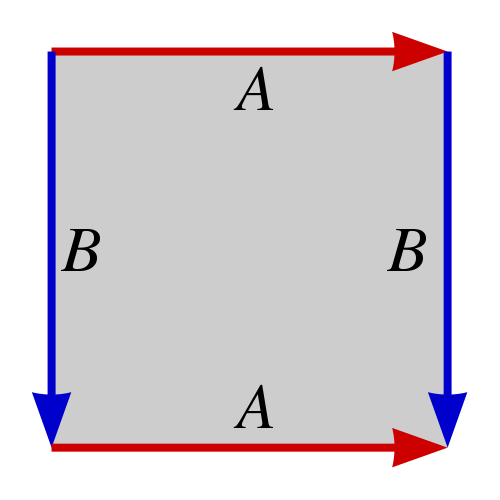
\includegraphics[width=0.3\textwidth]{torus}
\end{center}
\textbf{Answer: } The C-space for an Asteroids-style video game is homeomorphic to a torus $\mathbb{T}^2$. This is because when the spaceship crosses any edge of the screen, it is immediately transported to same point on the opposite edge of the screen. The torus' identification is shown above. 


\section{Problem 4.14}
\textbf{Question: }Quaternions:
\begin{enumerate}
\item Define a unit quaternion $ h_1$ that expresses a rotation of  $ -\frac{\pi}{2}$ around the axis given by the vector  $ [ \frac{1}{\sqrt
3} \;\; \frac{1}{\sqrt 3} \;\; \frac{1}{\sqrt 3} ]$.
\item Define a unit quaternion $ h_2$ that expresses a rotation of $ \pi $ around the axis given by the vector  $ [ 0 \;\; 1 \;\; 0 ]$.
\item Suppose the rotation represented by $ h_1$ is performed, followed by the rotation represented by $ h_2$. This combination of rotations can be represented as a single rotation around an axis given by a vector. Find this axis and the angle of rotation about this axis. 
\end{enumerate}

\textbf{Answer: } \begin{enumerate}
\item The translation from axis-angle to quaternion is given by the following equation 
\begin{equation*}
h = \cos \frac{\theta}{2} + \left( v_1 \sin \frac{\theta}{2} \right)i + \left(v_2 \sin\frac{\theta}{2} \right) j + \left( v_3 \sin \frac{\theta}{2} \right) k
\end{equation*} 
Applying this equation yields $h = \frac{1}{\sqrt{2}} -\frac{1}{\sqrt{6}}i -\frac{1}{\sqrt{6}}j -\frac{1}{\sqrt{6}}k $
\item Applying the same equation as above, the resulting quaternion is $h = 0 + 0i + 1j + 0k$
\item The combination of two quaternions is given below. It is important to note that this equation reverses the order of the complex and real components, using $q_1 = i, q_2 = j, q_3 = k, q_4 = \mathbb{R}$. Applying this quaternion multiplication yields 
\begin{equation}
q' = b\otimes a = \frac{1}{\sqrt{6}}i -\frac{1}{\sqrt{6}}j + \frac{1}{\sqrt{2}}k + \frac{1}{\sqrt{6}}
\end{equation}
\end{enumerate}

Converted back to axis-angle representation this rotation is about the axis $\begin{bmatrix}0.447, -0.447, 0.774\end{bmatrix}$ of approximately 2.3 rad.

\begin{equation*}
\mathbf{b}\otimes\mathbf{a} =
\left[ {\begin{array}{rrrr}
    a_4 &   a_3 & -a_2 &  a_1\\
   -a_3 &   a_4 &  a_1 &  a_2\\
    a_2 &  -a_1 &  a_4 &  a_3\\
   -a_1 &  -a_2 & -a_3 &  a_4
\end{array}} \right]
\left[ {\begin{array}{c}
   b_1\\
   b_2\\
   b_3\\
   b_4
\end{array}} \right] =
\left[ {\begin{array}{rrrr}
    b_4 &  -b_3 &  b_2 &  b_1\\
    b_3 &   b_4 & -b_1 &  b_2\\
   -b_2 &   b_1 &  b_4 &  b_3\\
   -b_1 &  -b_2 & -b_3 &  b_4
\end{array}} \right]
\left[ {\begin{array}{c}
   a_1\\
   a_2\\
   a_3\\
   a_4
\end{array}} \right]
\end{equation*}



\section{Problem 4.16}
\textbf{Question: } Suppose five polyhedral bodies float freely in a 3D world. They are each capable of rotating and translating. If these are treated as "one" composite robot, what is the topology of the resulting C-space (assume that the bodies are not attached to each other)? What is its dimension?
 
\textbf{Answer: } Each of the 5 bodies have three axes of translation. As such, the resulting C-space will include $\mathbb{R}^{3*5} = \mathbb{R}^{15}$. Then, each body has 3 degrees of rotation. As mentioned previously, $\mathbb{S}^2 \neq \mathbb{S} \times \mathbb{S}$. Instead we use the notation $\mathbb{T}^n = (\mathbb{S}^1)^n$. Five robots with 3 rotational DOF each yields $(\mathbb{S})^{3*5} = \mathbb{T}^{15}$

The resulting C-space for 5 independent, free bodies in $\mathbb{R}^3$ has 30 DOF total. 
\begin{equation}
\mathbb{R}^{15} \times \mathbb{T}^{15}
\end{equation}

\section{Implementation - Tables}
\begin{center}
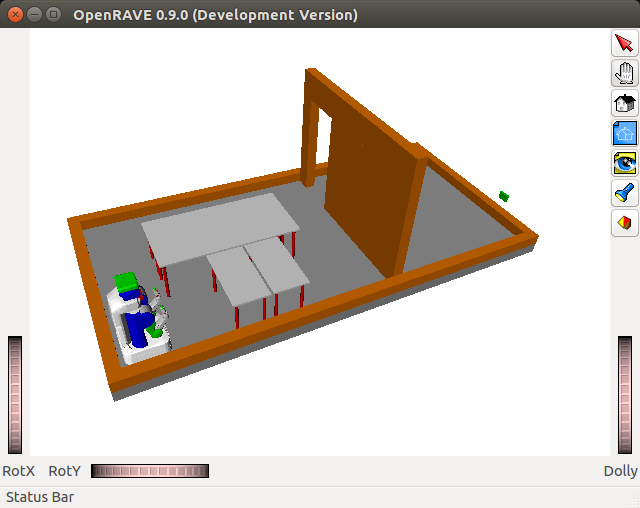
\includegraphics[width=0.5\textwidth]{HW1_tables_ss}
\end{center}

\section{Implementation - Puma}
\begin{center}
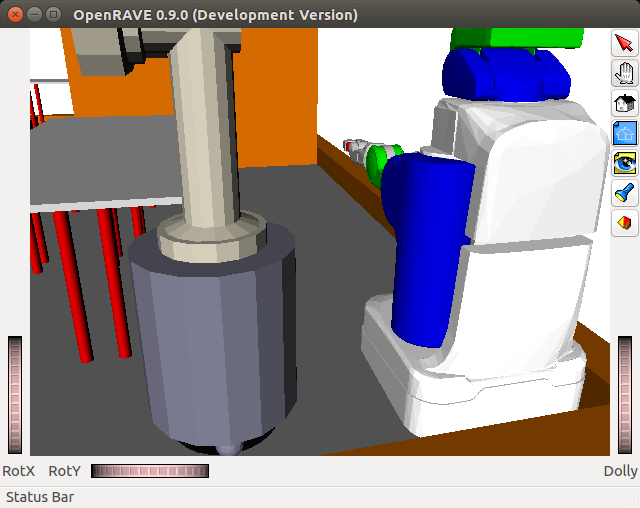
\includegraphics[width=0.45\textwidth]{HW1_puma_ss1}
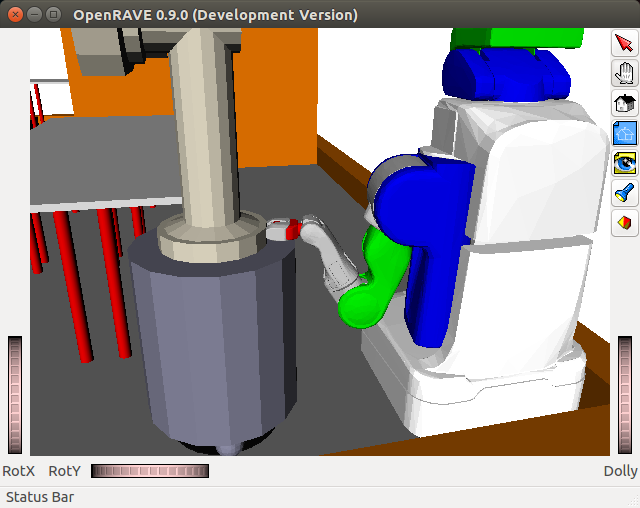
\includegraphics[width=0.45\textwidth]{HW1_puma_ss2}
\end{center}

\section{Implementation - Drawing}
\begin{center}
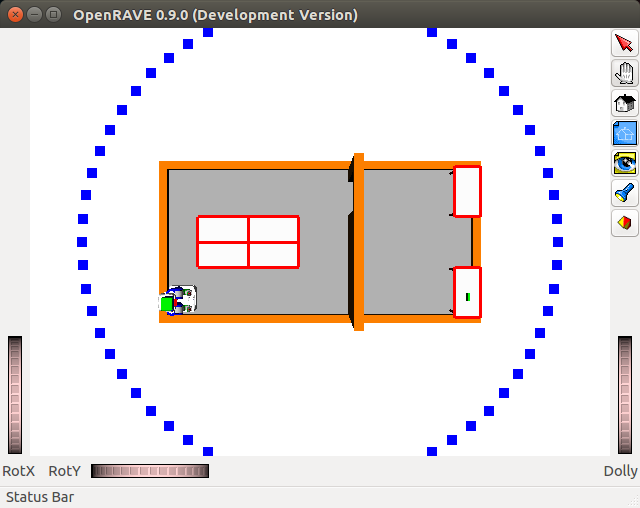
\includegraphics[width=0.5\textwidth]{HW1_drawing_ss}
\end{center}


\section{Implementation - Collision}
\begin{center}
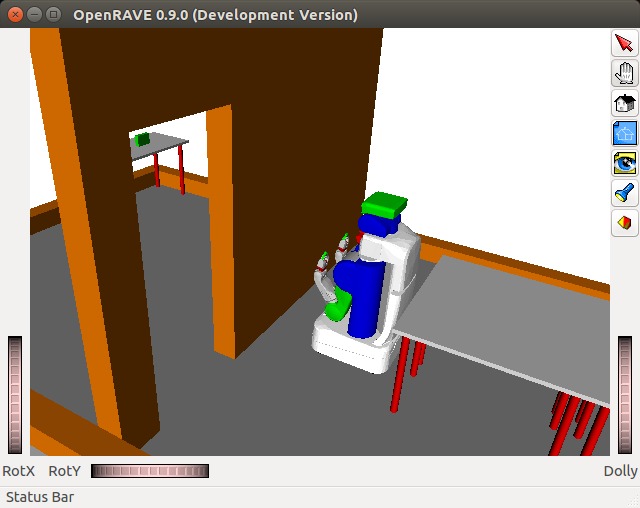
\includegraphics[width=0.45\textwidth]{HW1_collision_ss1}
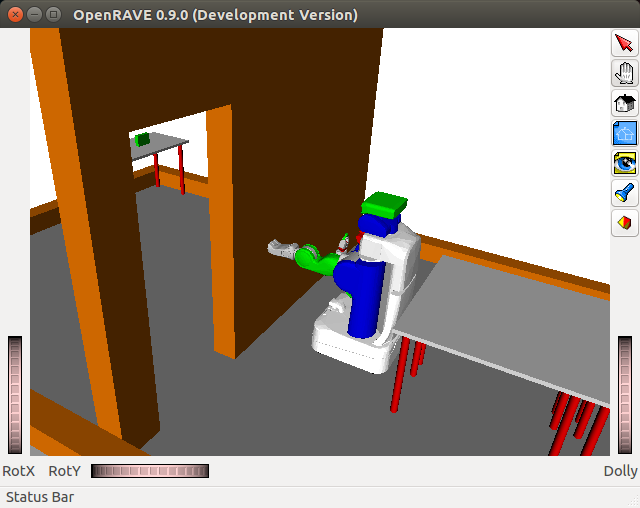
\includegraphics[width=0.45\textwidth]{HW1_collision_ss2}
\end{center}
An important note on implementation. When calling the waitrobot() function, it is important to call it \emph{outside} of the \begin{texttt}with env:\end{texttt} block. This prevents unnecessary locking of the scene-graph, and will prevent your program from hanging or crashing when multiple threads are trying to modify the \begin{texttt}env\end{texttt} variable. 

\end{document}



